\documentclass[hyperref={colorlinks=true}]{beamer}
\usepackage{hyperref}
\usepackage[utf8x]{inputenc}
\usepackage{euler}
\usepackage{listings}
\lstset{language=C++, basicstyle=\footnotesize}

%\usetheme{Berlin}
\usetheme[pageofpages=of,% String used between the current page and the
                         % total page count.
          bullet=circle,% Use circles instead of squares for bullets.
          titleline=true,% Show a line below the frame title.
          alternativetitlepage=true,% Use the fancy title page.
          %titlepagelogo=logotipo_pdf1,% Logo for the first page.
          %watermark=logotipo_pdf1,% Watermark used in every page.
          %watermarkheight=100px,% Height of the watermark.
          %watermarkheightmult=2,% The watermark image is 4 times bigger
                                % than watermarkheight.
          ]{Torino}

\title[M342]{M342 Álgebra Computacional}
\author{Christian Lomp}
\institute{FCUP}
\date{12 de setembro de 2011}
\begin{document}

\begin{frame}
\titlepage
\end{frame}

\section{1. Introdução}
\begin{frame}{1. Introdução}

 Aspectos computacionais de álgebra:

 \begin{itemize}
  \item\pause Representação de estruturas algébricas no computador;
  \item\pause Aritmética de  inteiros, corpos racionais, polinómios numa indeterminada;
  \item\pause Aritmética de matrizes e vectores;
  \item\pause Aritmética de polinómios em múltiplas indeterminadas;
  \item\pause Problemas de geometria algébrica (Bases de Gröbner).
 \end{itemize}
\pause Programação na linguagem C++. 
\end{frame}

\subsection{C++}
\begin{frame}{C++ versus Python}

{\it C++ é compilada:} 
\begin{center}\fbox{editar}$\longrightarrow$\fbox{compilar}$\longrightarrow$ \fbox{executar}\end{center}

{\it C++ é "strongly typed"}: 
\begin{center} \begin{itemize} \item variáveis têm de ser declaradas antes do primeiro uso e seu típo têm de ser especificado \item o valor da função tem ser declarado \end{itemize}\end{center}

\end{frame}

\begin{frame}{Compiladores e IDE}

\begin{itemize}
\item \pause  {\it Gnu CC}: compilador para todas as plataformas {\tiny \url{http:/gcc.gnu.org}}
\item \pause  {\it Code::Blocks} IDE para todas as plataformas {\tiny \url{http://www.codeblocks.org/}}
\item \pause {\it Microsoft Visual C++} IDE para Windows;  gratuito para alunos da UP 
{\tiny \url{https://sigarra.up.pt/up/WEB_BASE.GERA_PAGINA?P_pagina=1001525 }}
\item \pause  {\it Eclipse}: IDE para todas as plataformas;
\item \pause {\it Xcode}: IDE para Mac OS X
\end{itemize}
\begin{center}
\includegraphics{gnu.png}   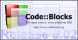
\includegraphics{CodeBlocks.png}   
\includegraphics{MSVisualC++.png}\end{center}
\end{frame}

\begin{frame}{Variáveis}
\begin{block}{Variáveis}
Espaço de memória reservado para armazenar tipos de dados, com um nome para referenciar seu conteúdo.
\end{block}
Observações importantes
\begin{itemize}
 \item Todas as variáveis devem ser declaradas antes de serem usadas.
 \item Mais de uma variável do mesmo tipo: separam-se seus nomes por vírgulas.
\end{itemize}
\end{frame}
\begin{frame}{Memória}
 
\begin{block}{Memória}
\begin{itemize}
\item  {\it 1 bit} = menor unidade de informação, dois valores $\{0,1\}$.
 \item {\it 1 byte} = 8 bit \fbox{$a_0$}\fbox{$a_1$}\fbox{$a_2$}\fbox{$a_3$}\fbox{$a_4$}\fbox{$a_5$}\fbox{$a_6$}\fbox{$a_7$}; representa o número
$$ 0 \leq \sum_{i=0}^7 a_i 2^i < 2^8=256$$
\end{itemize}
\end{block}

\end{frame}


%\subsection{Tipos de dados em C++}
\begin{frame}{Tipos de dados em C++}

C++ conhece os seguintes tipos de variáveis:
{\tiny 
\begin{center}\begin{tabular}{lllcc}
{\it tipo} & & nº bytes & valores & \\\hline\hline
{\it char} & caracter & 1 byte & $-128 \cdots  127$ & (signed)\\[3mm]
           &          &        & $0 \cdots 255$ & (unsigned)\\\hline
{\it short} & inteiro & 2 bytes & $-32768 \cdots 32767$ & (signed)\\[3mm]
  &  &  & $0 \cdots 65535$ & (unsigned) \\\hline
{\it int} & inteiro & 4 bytes & $-2.147.483.648 \cdots  2.147.483.647$ & (signed)\\[3mm]
 & &  & $0 \cdots 4.294.967.295 = 2^{32}-1$ & (unsigned) \\\hline
{\it long long} & inteiro & 8 bytes & $-9.223.372.036.854.775.808 \cdots  9.223.372.036.854.775.807$ & (signed)\\[3mm]
 & &  & $0 \cdots 18.446.744.073.709.551.615 = 2^{64}-1$ & (unsigned) \\\hline 
{\it bool } & v/f & 1 byte & {\it true} ou {\it false}&  \\\hline
{\it float} & ``real'' & 4 bytes & $\pm  3.4e^{\pm 38}$ (ca. 7 digitos)& \\\hline
{\it double} & ``real'' & 8 bytes & $\pm  1.7e^{\pm 308}$ (ca. 15 digits)&  \\\hline
\end{tabular}\end{center}}
\end{frame}


\begin{frame}[fragile]{Exemplo}
\begin{tabular}{ll}
{\it Python} & {\it C++} \\
\begin{minipage}{150px}
\begin{lstlisting}[language=Python]
a=3
b=a*a+2
print a,b
\end{lstlisting}
\end{minipage}
&
\begin{minipage}{150px}
\begin{lstlisting}[language=C++]
#include <iostream>
using namespace std;

int main() 
{
   int a=3;
   int b=a*a+2;
   cout << a << b;
}
\end{lstlisting}
\end{minipage}
\end{tabular}
\end{frame}

\begin{frame}[fragile]{Ciclo 'for'}

\begin{lstlisting}[language=C++]
#include <iostream>
using namespace std;

int main() 
{
   int n=10, factorial=1;  
   cin >> n;
   for (int i=1; i<=n; i++) 
     factorial=factorial*i;
   cout << factorial;
}
\end{lstlisting}

\end{frame}

\begin{frame}[fragile]{Ciclo 'while'}

\begin{lstlisting}[language=C++]
#include <iostream>
using namespace std;

int main() 
{
   int n=10, factorial=1, i=1;
   cin >> n;
   while(i<=n) { 
     i++;
     factorial=factorial*i;
   }
   cout << factorial;
}
\end{lstlisting}

\end{frame}

\begin{frame}[fragile]{Ciclo 'do while'}

\begin{lstlisting}[language=C++]
#include <iostream>
using namespace std;

int main() 
{
   int n=10, factorial=1, i=1;
   cin >> n;
   do { 
     i++;
     factorial=factorial*i;
   } while (i<n);   
   cout << factorial;
}
\end{lstlisting}

\end{frame}


\begin{frame}[fragile]{Funções}

\begin{lstlisting}[language=C++]
#include <iostream>
using namespace std;

int factorial ( int n )
{
  if (n==0)
    return 1;
  else 
    return n*factorial(n-1);
};

int main();
{
   int n=10;
   cin >> n;
   cout factorial(n);
}
\end{lstlisting}

\end{frame}


\begin{frame}{STL - Standard Template Library}

\begin{enumerate}
 \item Funções do input/output (io): manipulação de ficheiros, teclado, etc. (e.g. {\it cout, cin, ...}).
 \item Funções para manipular de {\it strings}.
 \item Classes para tratar de {\it listas}, {\it vectores}, {\it conjuntos}, {\it funções}, etc...
\end{enumerate}


\end{frame}


\begin{frame}[fragile]{Classes}

\lstset{ language=C++,         basicstyle=\tiny}

\begin{lstlisting}[language=C++]
#include <iostream>
using namespace std;

class inteiro 
{
  unsigned int n;
  public:
    inteiro (unsigned int numero) { n=numero; };

    unsigned int factorial() { 
      unsigned int fact=1;  
      for (int i=1; i<=n; i++)   fact=fact*i;
      return fact;
    }    
};

main() {
  unsigned int n;
  cin >> n;
  inteiro numero(n);
  cout << numero.factorial() << endl;
}

\end{lstlisting}
 
\end{frame}


\begin{frame}[fragile]{Classes}

\begin{lstlisting}[language=C++]
 
class triangulo {
  
  int a,b,c ;
  public:

  triangulo (int lado1, int lado2, int lado3) { 
     a=lado1;  b=lado2;  c=lado3;
  }

  double Area() { ...  };    
};

main() {
  triangulo t(3,4,5);
  cout << t.Area()<< endl;
}

\end{lstlisting}
 
\end{frame}




\end{document}
